\chapter{On-Chain Design}

\section{Blockchain Platform and Technologies}
The development of a blockchain-based system begins with the selections of a suitable blockchain platform. We selected \acrlong{eth}, a public blockchain known for its extensive developer community and rich ecosystem of features particularly suitable for an academic record systems \cite{mustafa2024publiceduchain}\cite{yassynzhanbolatzhan2021verificationuniversitystudent}. \acrlong{eth} supports smart contract development in multiple languages and serves as the foundation for various layer 2 solutions that enhance performance and scalability. This flexibility allows the system to be initially developed for the \acrlong{eth} mainnet and later migrated to a layer 2 chain to take advantage of specific features, with minimal development overhead. Notable \acrlong{eth}-based layer 2 solution include:

\begin{itemize}
    \item \textbf{Polygon}, offering faster and more cost-efficient transactions than the Ethereum mainnet.
    \item \textbf{Arbitrum}, improving scalability while maintaining compatibility with Ethereum smart contracts.
    \item \textbf{ZKsync}, ensuring high security and rapid finality through validity proofs.
    \item \textbf{Optimism}, emphasizing simplicity and seamless integration with the Ethereum ecosystem.
    \item \textbf{Starknet}, introducing its own high-performance language, Cairo\footnote{\url{https://www.cairo-lang.org/}}, optimized for zero-knowledge computation.
\end{itemize}

For the implementation, we selected Solidity\footnote{\url{https://soliditylang.org/}} as the programming language. Solidity is an object-oriented language, designed specifically for writing smart contracts on \acrlong{eth} and the \acrshort{evm}, influenced by C++, JavaScript and Python\footnote{\url{https://github.com/ethereum/solidity/blob/develop/docs/index.rst}}. It is the most widely adopted language in the \acrlong{eth} ecosystem, supported by and active and large developer community. Given our prior experience with Solidity, this choice was natural and well-suited to our objectives.

\section{Architecture}
\begin{figure}
  \centering
  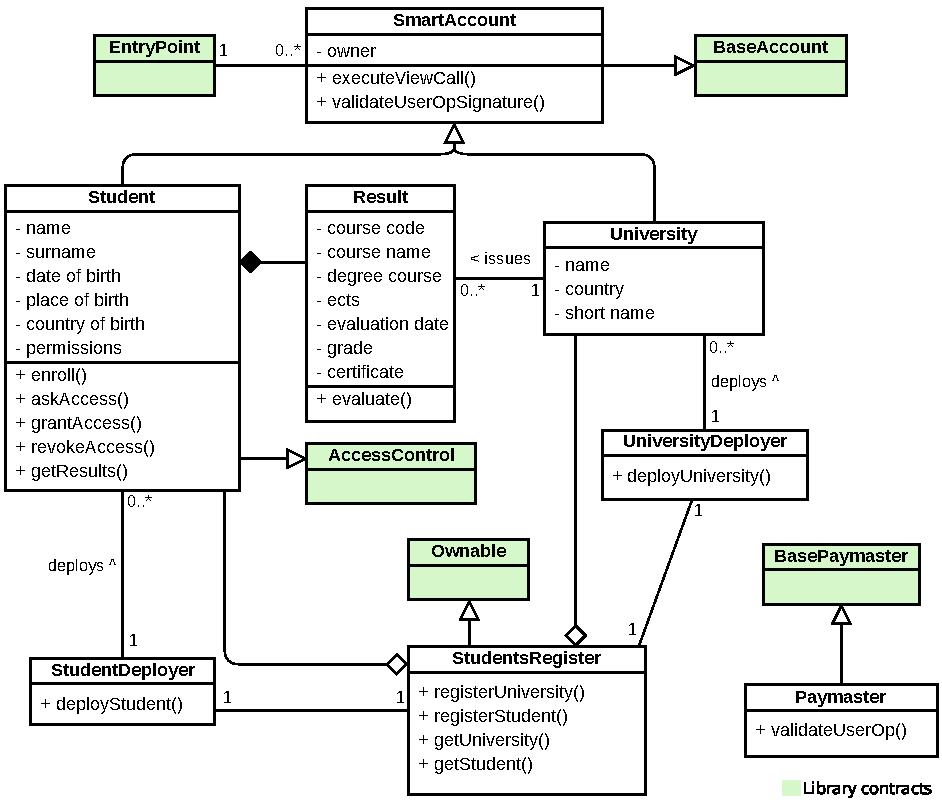
\includegraphics[width=1\textwidth]{figures/Contracts class diagram.pdf}
  \caption[Smart contracts architecture class diagram]{Class diagram representing smart contracts architecture}
  \label{fig:contractsClass}
\end{figure}

The overall architecture of the system is illustrated in the class diagram in \cref{fig:contractsClass}. The \acrshort{ew} system is composed of seven custom smart contracts, represented as white classes in the diagram. (\textit{Result} is not a smart contract, see \cref{ssec:studentContract} for more details). 

\begin{enumerate}
    \item \textbf{SmartAccount}: Defines the structure of a smart account following the account abstraction protocol.
    \item \textbf{Student}: Represents an individual student in the system.
    \item \textbf{University}: Represents a university entity.
    \item \textbf{StudentDeployer}: Responsible for deploying \textit{Student} contracts.
    \item \textbf{UniversityDeployer}: Deploys \textit{University} contracts.
    \item \textbf{StudentsRegister}: Manages and stores information about students and universities.
    \item \textbf{Paymaster}: Sponsors blockchain transactions made by students and universities.
\end{enumerate}
It addition, the system relies on four external contracts, shown in green in \cref{fig:contractsClass}, which are derived from established libraries such as \textit{OpenZeppelin}\footnote{https://openzeppelin.com/}:
\begin{enumerate}
    \item \textbf{EntryPoint}: A singleton contract that receives transactions from smart accounts and executes user operations.
    \item \textbf{AccessControl}\footnote{\url{https://docs.openzeppelin.com/contracts/5.x/access-control}}: Provides a comprehensive role-based access control mechanism.
    \item \textbf{BaseAccount}: Abstract contract defining the core behaviors of a smart account under the account abstraction protocol.
    \item \textbf{BasePaymaster}: Abstract contract defining the structure of a paymaster that sponsors user transactions.
\end{enumerate}

\subsection{SmartAccount}

\subsection{Student}
\label{ssec:studentContract}
The \textit{Student} contract encapsulates the majority of the system's logic. Its primary responsibilities include storing the student's personal information, such as name, surname, date of birth, place of birth and country of birth, as well as managing their academic records. These records are stored using the structure presented in \cref{lst:resultStruct}. 
\lstinputlisting[
    caption={\textit{Result} structure within the \textit{Student} smart contract},
    label=lst:resultStruct,
    language=Solidity,
]{listings/result.sol}
Due to Solidity's limited support for floating-point numbers, and because the \acrshort{ects} credits may not always be whole number, the \acrshort{ects} value is stored as the original number multiplied by 100. The type \textit{uint16} is used for this purpose, allowing values up to 655.36\footnote{The maximum number representable with 16 bits is 65536},  which is more than sufficient for academic credit systems. A smaller unsigned integer type, such as \textit{uint8}, supports only values from 0 to 2.55 in this context, which is clearly inadequate. The field \textit{certificateHash} stores the CID of the certificate, acting as a reference to its location in the decentralized storage system (see BACKGROUND\_IPFS and \cref{sec:decStorageDesgn} for further explanation). 

Additional functionalities, all addressing \textit{FR 5} in \cref{tab:funcReq}, include enabling universities to:
\begin{itemize}
    \item Retrieve a student's personal and academic information.
    \item Enrol the student in a new course.
    \item Record and evaluation for course the student has already attended.
\end{itemize}
All such interactions are governed by a strict access control mechanism, implemented to fulfill the relevant functional requirements outlined in \cref{tab:funcReq}, namely \textit{FR 6}, \textit{FR 7}, and \textit{FR 12}. This mechanism is based on the \textit{AccessControl} library, specifically the \textit{AccessControlEnumerable} variant, which enables the definition of roles and their association with specific addresses. Within the \textit{Student} contract, four distinct roles are defined:

\begin{enumerate}
    \item \textbf{reader}
    \item \textbf{writer}
    \item \textbf{reader requester}
    \item \textbf{writer requester}
\end{enumerate}
These roles cover all possible scenarios. When an institution requests read or write access to a student's academic records,  its smart account address is assigned the corresponding role. Since \textit{AccessControlEnumerate} supports enumeration of role bearers, the student can query and view which institutions have pending access requests. When an institution attempts to access or modify a student's academic records, the \textit{Student} contract verifies whether the caller's address has been granted the appropriate role, thereby enforcing access restrictions. This mechanism requires the \textit{Student} contract to support a set of permission management functions, including the ability for students to grant, revoke, and inspect permissions (\textit{FR 12}), as well as for universities to request and verify their access rights (\textit{FR 7}).

As shown in \cref{fig:useCaseCli}, \textit{Student} contracts are deployed by the \textit{StudentDeployer}, which is invoked by the \textit{StudentsRegister} contract when a university registers a new student in the \acrshort{ew} system. Upon registration, the initiating university is automatically granted write permissions for the student's academic record, reflecting its role as the enrolling institution responsible for issuing evaluations. All subsequent interactions with the \textit{Student} contract are carried out either by the browser extension or the \acrshort{sdk}. The browser extension is responsible for retrieving personal and academic data and managing permissions on the student's behalf. The \acrshort{sdk}, on the other hand, acts on behalf of universities to access and modify the student's academic wallet. To facilitate these interactions, the \textit{Strudent} contract defines several structured data types, which are used for functions inputs and outputs. These structures improve code readability and usability by grouping related data into cohesive types. Instead of requiring users to  pass multiple separate parameters in a specific order, an approach that increases the risk of errors, developers can simply import the relevant structure and populate its fields. The data type defined in the \textit{Student} contract are:

\begin{itemize}
    \item \textbf{EnrollmentInfo}: Contains the information required to enrol a student in a course; used as input for the enrolment function.
    \item \textbf{EvaluationInfo}: Contains the data needed to record an evaluation; used as input for the evaluation function.
    \item \textbf{Result}: Previously presented, this structure stores the details of a course attended by the student and is used to return the student's academic records.
    \item \textbf{StudentBasicInfo}: Represents the student's personal information.
    \item \textbf{StudentInfo}: A composite structure that includes the \textit{StudentBasicInfo} and a list of \textit{Result} structures, representing the student’s complete academic profile.
\end{itemize}

\subsection{University}
Since the primary focus of this work is on the interaction between students and their academic records, as well as the ownership of such data, the institutional accounts (smart accounts) of universities, implemented through the \textit{University} contract, are designed to simpler that those of students. The \textit{University} contract, like \textit{Student}, extends the \textit{BaseAccount} contract, enabling it to function as a smart account compatible with the account abstraction protocol. As a result, universities can use their institutional wallet, via the \acrshort{sdk}, to perform blockchain transactions, which are then sponsored by the \textit{Paymaster}. 

In addition, because universities are identified solely by their contract address in interactions with other smart contracts, the \textit{University} contract also stores descriptive metadata, including the institution's name, country, and a short identifier. Apart from the \textit{UniversityDeployer}, which is responsible for deploying the contract, the only components that interact directly with the \textit{University} contract are the \acrshort{sdk} and the browser extension. When these components need to access university-related information, they do so using the institution's contract address. For instance, when a student retrieves their academic records, each record references the issuing university by it address. The browser extension must then query the blockchain to access the corresponding \textit{University} contract and extract the relevant metadata.    

\subsection{StudentDeployer and UniversityDeployer}
The deployment of \textit{Student} and \textit{University} contracts is handled by the \textit{StudentDeployer} and \textit{UniversityDeployer} contracts, respectively. When a system administrator registers a new university, or a university registers a new student through the \acrshort{sdk}, they interact with the \textit{StudentsRegister} smart contract. This contract, in turn, invokes one of the deployer contracts to create the corresponding smart contract instance. This architecture implements the factory pattern, a design principle commonly used in object-oriented programming to abstract the creation of objects. In the context of the \acrshort{ew} system, the deployer contracts abstract and encapsulate the instantiation of new \textit{Student} and \textit{University} contracts.

The adoption of the factory pattern offers several advantages over embedding the deployment logic directly within the \textit{StudentsRegister} contract:

\begin{itemize}
    \item It separates the contract creation logic from the registration logic, improving modularity and maintainability.
    \item It reduces the complexity of the \textit{StudentsRegister} contract by externalizing the deployment process.
    \item It minimizes the contract size of \textit{StudentsRegister}. In Solidity, deploying a contract via the \texttt{new} keyword requires embedding the bytecode of the deployed contract, which increases the size of the calling contract. Since Solidity enforces a maximum contract size of 24576 bytes, including large deployment code directly could exceed this limit. Using external deployer contracts bypass this issue.
\end{itemize}

The decision to centralize deployments through the \textit{StudentsRegister} contract was also motivated by gas efficiency. On blockchain platforms, reducing the number of transactions typically leads to lower gas costs. By combining the deployment of a contract and the registration of its address into a single transaction, the system reduces the overall gas consumption required for onboarding new entities.

\subsection{StudentsRegister}

\subsection{Paymaster}
One of the system's key feature is that blockchain usage is nearly transparent for users. Students do not directly interact with wallets or perform transactions themselves, and universities only need the private key associated with their \acrshort{eth} account to manage their institutional smart wallet. This level of abstraction is made possible by the \textit{Paymaster}, a smart contract deployed on the blockchain that sponsors all transactions made by users. This design directly readdressing \textit{NFR 5} (see \cref{tab:nonFuncReq}), which emphasizes minimizing the complexity of interactions with the system for end users.

Without the \textit{Paymaster}, the system would require a mechanism to fund user wallets, presenting three primary options:

\begin{enumerate}
    \item Each user funds their own wallet.
    \item Universities fund the wallets of both students and themselves.
    \item The \acrshort{ew} system centrally manages and funds all wallets.
\end{enumerate}
Each approach has significant drawbacks. The first and second require users to manage cryptocurrency wallets and purchase tokens, which increases complexity and cost, especially burdensome for students. The third alternative still introduces administrative overhead and security concerns related to managing a large number of wallets.

Our solution utilizes a \textit{Paymaster} that implements the \textit{BasePaymaster} abstract contract, developed as part of the ERC-4337 protocol\footnote{\url{https://www.erc4337.io/}}. For simplicity, our current implementation sponsors all user operations (transactions) it receives, without validating their origin or gas cost. The only enforced constraint, inherited from \textit{BasePaymaster}, is that transactions must be routed through a known \textit{EntryPoint} contract.
This configuration is suitable for testing environments such as local or test networks, where there is no risk of losing real tokens. In a real-world deployment, a more robust implementation would be necessary, specifically, one that integrates with the \textit{StudentsRegister} contract to verify that the transaction sender is a verified student or university. 